\documentclass[a4paper]{jarticle}
\usepackage{sf}

%図に関する設定
\usepackage[dvipdfmx]{graphicx}
\graphicspath{{0.Fig/}}
\renewcommand{\figurename}{Fig.}
\usepackage{caption}%図のキャプションの幅
\usepackage{float} %図の位置を強制的に指定するためのパッケージ
% \setlength{\textfloatsep}{3pt} % 図と本文の間の余白を5ptに設定
% \setlength{\intextsep}{3pt}    % 図と本文の間の余白を5ptに設定
\usepackage{placeins}
%数式に関する設定
\usepackage{amsmath}
%添削時の色の設定%{\color{red} 赤色の文字}で使う
\usepackage{xcolor} 
% %セクションの行間を狭くしたい
% \usepackage{titlesec}
% \titleformat{\section}[block]{\centering\normalfont\Large\bfseries}{\thesection}{1em}{} % セクションを中央揃え
% \titlespacing*{\section}{0pt}{10pt}{5pt} % \sectionの余白設定
% \titlespacing*{\subsection}{0pt}{7pt}{5pt} % \subsectionの余白設定

\title{柔軟物モデルとアクティブセンシングに基づいた\\軌道生成によるセンサレス反力推定}
\author{○金谷 孝一郎$^1$, 村上 健一$^2$, 山川 雄司$^3$}
\affiliation{
$^1$ 東京大学,
$^2$ 東京大学,
$^3$ 東京大学 }
\Etitle{Sensorless Reaction Force Estimation through Trajectory Generation \\ Based on Deformable Object Modeling and Active Sensing}
\Eauthor{○Koichiro Kanaya , Kenichi Murakami and Yuji Yamakawa  }
\Eaffiliation{
$^1$ University of Tokyo,
$^2$ University of Tokyo,
$^3$ University of Tokyo }
\Abstract{%日本語アブストラクト(本文が英語の場合は英語でも可).200字程度で記載.
% 本研究では、柔軟物の粘弾性パラメータを推定し,力センサを用いずに接触力を推定する手法を提案する.
本研究では,力センサを用いずにグリッパと柔軟物間の反力を推定するために,バネとダンパでモデル化した柔軟物のパラメータ同定法を提案する.
提案手法では、アクティブセンシングに基づきグリッパの軌道を生成し,ノイズにロバストな同定計算を行う.
実験では,鶏むね肉や豆腐,バナナを対象に,提案手法の反力推定精度を評価した.その結果,単純な5次関数のグリッパ軌道と比較して推定精度が向上することを確認した.
% 本手法は,柔軟物の把持や操作をセンサレスで実現する基盤技術として有用である.
}

\begin{document}
\maketitle
\iffalse
\section{原稿の書き方}
\begin{itemize}
\item 原稿枚数はA4版で4~6ページです.超過しないようご注意下さい.
\item 用紙余白は上下24mm,左右15mmとし,本文を縦250mm×横180mmの枠内に収めて下さい.
\item 冒頭に以下の項目を書いてください.
\begin{itemize}
\item 一行目:和文題目.
\item 二行目:和文著者名.登壇者の前に必ず○をつけてください.
\item 三行目:和文所属名.
\item 四行目:英文題目.
\item 五行目:英文著者名.登壇者の前に必ず○をつけてください.
\item 六行目:英文所属名.
\item 七行目以降:要旨(日本語.論文の本文が英文の場合,英語でも結構です)
\end{itemize}
\item 原稿はPDF形式で作成してください.印字の正確性を期すため,PDFファイル作成時にフォントの埋め込みをお願い致します.
\item 引用は文献\cite{ref1}のように記載してください.
\end{itemize}
\begin{thebibliography}{9}
\bibitem{ref1}
計測 太郎:センシングフォーラム予稿の書き方,
第39回センシングフォーラム論文集,pp. 1-5, 2022.
\end{thebibliography}
\section{図の挿入例}
以下にPDF形式の図を挿入します。

\begin{figure}[htbp]
    \centering
    \includegraphics[width=0.5\textwidth]{example.pdf}
    \caption{サンプル図}
    \label{fig:sample}
\end{figure}

図~\ref{fig:sample}はサンプル図です。
\fi

%%%%%%%%%%%%%%%%%%%%%%%%%%%%%%%%%%%%%%%%%%%%%%%%%%%%%%%%%%%%%%%%%%%%%%%%%%%%%%%%%%%%%%%%%%%%%%%%%%%%%%%%%%%%%%%%%%%%%%%%%%%%%%%%%%%%%%%%%%%%%%%%%%%%%
\section{緒言}
 近年,医療分野では患者と医師双方にメリットがある低侵襲手術が注目されている\cite{MIS_ref1}.従来の開腹手術と比較し,低侵襲手術は小さな皮膚切開を介して手術を行う.
これにより,患者には手術リスク,感染症リスクの低下\cite{MIS_ref2}や入院期間\cite{MIS_ref3},回復期間の短縮\cite{MIS_ref4}といったメリットがある.
また,外科医にも手術時の肉体的疲労の低減や,X線透視装置を用いた手術では,放射線被曝の低減といったメリットがある\cite{MIS_ref5}.

しかし,低侵襲手術に用いられる鉗子グリッパは,スペース的な制約\cite{MIS_ref1}や生体適合性の需要\cite{MIS_ref6}から,力センサを搭載することが難しい.
この力センサの不在は,外科医の練習期間の長期化\cite{MIS_learning_time}や,ロボットによる自動化を推進する上での課題となっている\cite{RMIS}.
鉗子グリッパへの力センサ搭載が困難である主な要因は,その小型化,生体適合性,殺菌処理への耐久性にある\cite{MIS_ref7}.
鉗子グリッパ内の限られた空間内では,力センサとその計測に必要な配線を組み込む物理的なスペースが不足する\cite{MIS_ref1}.
また,力センサが必ずしもチタンやステンレスといった生体適合素材で構成されるとは限らない\cite{MIS_ref6}.
さらに,鉗子グリッパは高温の蒸気により殺菌され,数回の殺菌処理によりセンサの精度が低下する\cite{MIS_ref7}.
% これらの要因による力センサの不在を解決するために,鉗子グリッパに搭載可能な力センサの開発\cite{?}や,力センサを用いないで接触力を推定する研究\cite{?}が行われており,本研究は後者に該当する.
これらの要因による力センサの不在を解決するために,力センサを用いないで反力を推定する技術には需要がある.

 推定反力は触覚フィードバックに使用され,ロボットを用いた自動化では,最低0.5 kHz\cite{fps_ref1},理想的には,1 kHzの更新頻度が必要とされる\cite{fps_ref2}.
この更新頻度を満たすために,反力推定での計算効率が重要である.本研究では臓器等の柔軟物を計算コストの小さいバネとダンパでモデル化し,バネ定数と粘性減衰係数を同定し,反力推定を行う.

%%%%%%%%%%%%%%%%%%%%%%%%%%%%%%%%%%%%%%%%%%%%%%%%%%%%%%%%%%%%%%%%%%%%%%%%%%%%%%%%%%%%%%%%%%%%%%%%%%%%%%%%%%%%%%%%%%%%%%%%%%%%%%%%%%%%%%%%%%%%%%%%%%%%%
\section{関連研究}
 センサレスで反力推定をする研究と,柔軟物をモデル化しロボットで操作する研究について述べる.
センサレスで反力推定をする研究には,内視鏡画像から反力を推定する研究と,駆動用モータやワイヤから反力を推定する研究がある.
まず,画像ベースの研究に関して,
ChuaらはRGB画像とロボットの状態をニューラルネットワークの入力とすることで,画像のみやロボットの状態のみを入力とする場合より,汎化能力を向上させた\cite{ref_Chua}.
さらに,単一フレームごとに反力を推定することで,37.7 Hzの更新速度を達成し,
リカレントニューラルネットワーク(12.4 Hz)と比較して,高速な反力推定を実現した.しかし,学習系を用いた手法では,1 kHzの更新頻度を達成することが難しいと考える.
Wangらは変形前後の画像から変位を計測し,既知の材料特性と有限要素法を用いて,力の位置と大きさを推定した\cite{ref_Wang}.変位の推定精度が反力推定精度に影響し,高制度な変位計測には,マーカが必要となるという課題がある.

駆動用モータやワイヤから推定する研究に関して,
Xueらは,ワイヤ駆動する鉗子グリッパをケーブルプーリーシステムでモデル化し,張力伝達特性,エンドエフェクタのカップル特性,隣接するプーリーの摩擦特性を考慮し,鉗子の把持力を推定した\cite{ref_Xue}.
しかし,グリッパが停止しているときの反力は停止前の値を取り続けるというアルゴリズムであり,塑性変形が進む柔軟物の反力を推定することは難しいと考える.

次に,柔軟物をモデル化しロボットで操作する研究は,柔軟物のモデル化に関して大きく3つに分類できる\cite{ref_review_modeling}.
1;柔軟物をバネとダンパでモデル化する研究,2;柔軟物を有限要素法でモデル化する研究,3;Position Based Dynamics(PBD)でモデル化する研究である.
まず,バネとダンパによりモデル化する手法は,計算量が少ない一方で,柔軟物の変形に対するモデルの精度が低い手法である\cite{ref_MSD}.
しかし,モデルのパラメータを同定する上で,柔軟物全体の変形を計測するだけでよいので内視鏡画像やグリッパのエンコーダによる計測が可能である.
次に,有限要素法でモデル化する手法は,柔軟物の変形に対するモデルの精度が高い\cite{ref_FEM}.しかし,計算量が多く,リアルタイムでの反力推定には不向きであり,密度やヤング率,ポアソン比を事前に計測する必要がある.
最後に,PBDでモデル化する手法は,柔軟物の変形に対するモデルの精度はバネダンパより高く,計算量は有限要素法よりも少ない\cite{ref_PBD}.しかし,柔軟物のせん断変形を計測する必要があり,マーカが必要となるが,臓器が出血することを考慮すると画像計測は難しいと考える.

% 本研究では,マーカレスと高い計算効率を重視し,柔軟物をバネとダンパでモデルを用い,力センサなしで柔軟物からの反力を推定する.
力センサを搭載していないグリッパは,エンコーダをもとに制御される.そのためグリッパが目標位置に到達し停止すると,制御入力である力入力は0 [N]になる.
しかし,柔軟物の変形に伴い反力は変化し,力入力だけでは反力推定することが困難である.
加えて,計算コストの低減や,マーカを用いず画像やエンコーダのみで計測を完結したいという需要がある.
そこで,本研究では柔軟物をバネとダンパでモデル化し,同定精度を向上させるために,グリッパが停止するまでの軌道を分割して生成する手法を提案する.
%%%%%%%%%%%%%%%%%%%%%%%%%%%%%%%%%%%%%%%%%%%%%%%%%%%%%%%%%%%%%%%%%%%%%%%%%%%%%%%%%%%%%%%%%%%%%%%%%%%%%%%%%%%%%%%%%%%%%%%%%%%%%%%%%%%%%%%%%%%%%%%%%%%%%
\section{課題設定}
 反力推定は変形段階と停止段階の2段階で行う.
まず変形段階では,グリッパの目標位置と制御入力である力入力からバネ定数,粘性減衰係数を同定する.
次に停止段階では,同定したバネ定数,粘性減衰係数とグリッパのエンコーダの値を用いて反力を推定する.

本研究は変形段階でのグリッパ軌道や同定計算に重きを置き,手法を提案する.
研究目的は,停止段階での推定反力を力センサの計測値に近づけることである.
%%%%%%%%%%%%%%%%%%%%%%%%%%%%%%%%%%%%%%%%%%%%%%%%%%%%%%%%%%%%%%%%%%%%%%%%%%%%%%%%%%%%%%%%%%%%%%%%%%%%%%%%%%%%%%%%%%%%%%%%%%%%%%%%%%%%%%%%%%%%%%%%%%%%%
\section{提案手法}
 弾性と塑性の両方の性質を表現する柔軟物モデルとして,図~\ref{fig:BS_model}に示すバーガースモデルが用いられる\cite{ref_MSD}.
図~\ref{fig:BS_model}のモデルの反力$f(t)$と,変形量$x(t)$の関係は以下のように表される.
\begin{equation}
    % \frac{k_1 k_2}{c_2}\int{x}\,dt + k_1 x = \frac{k_1k_2}{c_1 c_2}\iint{f}\,dt\,dt + \frac{k_1}{c_2}(1+\frac{k_2}{k_1}+\frac{c_2}{c_1})\int{f}\,dt + f
    p_1 {x} + p_2 \int{x}\,dt = p_3\int{f}\,dt +p_4\iint{f}\,dt\,dt  + f
    \label{eq:BSmodel}
\end{equation}
ここで,
\begin{equation}
    \begin{aligned}
        p_1 &= k_1,  \\
        p_2 &= \frac{k_1 k_2}{c_2},    \\
        p_3 &= \frac{k_1}{c_2}\left(1+\frac{k_2}{k_1}+\frac{c_2}{c_1}\right),\\
        p_4 &= \frac{k_1k_2}{c_1 c_2} ,\\
    \end{aligned}
    \label{eq:p2ck}
\end{equation}
である.
\begin{figure}[tb]
    \centering
    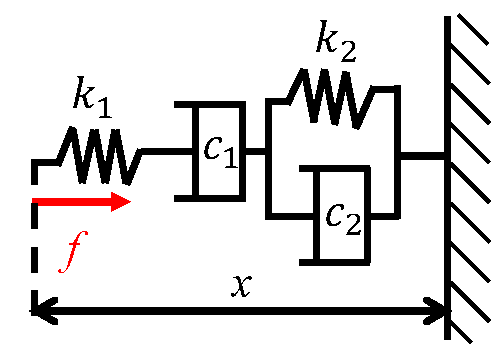
\includegraphics[width=0.3\textwidth]{BS_model.pdf}
    \caption{Bargers model.}
    \label{fig:BS_model}
\end{figure}
$k_1$,$k_2$は弾性係数であり,$c_1$,$c_2$は粘性減衰係数である.以降これらをまとめて粘弾性係数と呼び,時間積分$\int \,dt, \iint \,dtdt $は$\int, \iint$と表記する.
% 反力$f$はモータの力入力を用い,変形量$x$は接触後のグリッパの目標軌道を用いて,$p_1$,$p_2$,$p_3$,$p_4$を同定し,$k_1$,$k_2$,$c_1$,$c_2$を求める.
式~(\ref{eq:BSmodel})をタイムステップごとに行に格納し,行列形式で表すと,
\begin{equation}
    \mathbf{M}\mathbf{p} = \mathbf{q} 
    \label{eq:Mp_q}
\end{equation}
となる.ただし,
\begin{equation}
    \begin{aligned}
        \mathbf{M}_{n \times 4} &= \begin{bmatrix}
            \boldsymbol{x}, & \int{\boldsymbol{x}}, & -\int{\boldsymbol{f}}, & -\iint{\boldsymbol{f}}\\
        \end{bmatrix}, \\
        \mathbf{p}_{4 \times 1}  &= \begin{bmatrix}
            p_1 ,p_2 ,p_3 ,p_4
        \end{bmatrix}^{\mathrm{T}}, \quad
        \mathbf{q}_{n \times 1}   = \boldsymbol{f}
    \end{aligned}
\label{eq:BSmodel_matrix}
\end{equation}
である.
% 粘弾性係数$k_1$,$k_2$,$c_1$,$c_2$を同定することは,行列$\mathbf{M}$の擬似逆行列を算出する問題に帰着する.
行列$\mathbf{M}$の擬似逆行列を算出することで,粘弾性係数$k_1$,$k_2$,$c_1$,$c_2$を同定できる.
しかし,エンコーダの計測結果には,ノイズが含まれ,位置制御するモータの力入力には,ゲインが乗じられたノイズが現れる.
このノイズにより粘弾性係数の同定精度が低下するという課題がある.

この課題を解決するために,まず,\ref{subsec:QR_traj_and_calculation}節では,行列$\mathbf{M}$の特異値に着目し,
ノイズにロバストなグリッパの軌道生成方法と,その軌道に適した計算方法について述べる.
次に,\ref{subsec:downsample}節では,粘弾性係数が0や無限大に近づくことを防ぐために,粘弾性係数の更新方法について述べる.
これらの手法は変形段階での提案であり,グリッパが柔軟物と接触してから停止するまでの間,グリッパと柔軟物は接触を保つとする.
%%%%%%%%%%%%%%%%%%%%%%%%%%%%%%%%%%%%%%%%%%%%%%%%%%%%%%%%%%%%%%%%%%%%%%%%%%%%%%%%%%%%%%%%%%%%%%%%%%%%%%%%%%%%%%%%%%%%%%%%%%%%%%%%%%%%%%%%%%%%%%%%%%%%%%%%%%%%%%%
\subsection{QR分解を用いたグリッパの軌道生成と軌道に適した同定計算}\label{subsec:QR_traj_and_calculation}
 $\mathbf{M}$の特異値に注目し,ノイズにロバストな軌道を複数のサイクルに分割して生成する.
本節では,1;ノイズにロバストな特異値の決定方法,2;各サイクルでのQR分解を用いたグリッパの軌道生成方法,3;軌道に適した同定計算方法について述べる.

まず,ノイズを明示的に扱うために,$\mathbf{q}$のノイズを$\mathbf{noise}$とする.
$\mathbf{p}$の算出は,行列$\mathbf{M}$の擬似逆行列$\mathbf{M}^{\dagger}$を用いて,
\begin{equation}
    \begin{aligned}
    \mathbf{M}\mathbf{p} &= \mathbf{q} + \mathbf{noise}\\
              \mathbf{p} &= \mathbf{M}^{\dagger}(\mathbf{q} + \mathbf{noise})\\ 
            %   \mathbf{p} &= \sum \frac{1}{\gamma}vu^T(\mathbf{q}+\mathbf{noise})\\
            \mathbf{p} &= \mathbf{V}\mathbf{\Sigma}^{-1}\mathbf{U}^T(\mathbf{q}+\mathbf{noise})\\
    \end{aligned}
\end{equation}
のようになる.ただし,
\begin{equation}
            \mathbf{\Sigma}^{-1} =
            \begin{bmatrix}
                 \mathrm{diag}(\frac{1}{\gamma}, \frac{1}{\gamma}, \frac{1}{\gamma}, \frac{1}{\gamma}), \mathbf{0}_{4 \times n}
            \end{bmatrix}
\end{equation}
である.ここで,$\mathbf{V},\mathbf{U},\gamma$は行列$\mathbf{M}$を特異値分解したときの直交行列と特異値であり,$\gamma$を
\begin{equation}
    \mathrm{O}(\min({\mathbf{p}})) \gg \frac{\mathrm{O}(\mathbf{noise})}{\mathrm{O}(\mathbf{\gamma})}
    \label{eq:gamma}
\end{equation}
のように決定することでノイズの影響を抑えた$\mathbf{p}$の算出ができる.

次に,行列$\mathbf{M}$の特異値$\gamma$が式~(\ref{eq:gamma})を満たすように,グリッパの軌道$\boldsymbol{x}$をQR分解を用いて生成する.図~{\ref{fig:QR_traj}}にその概略を示す.
$\boldsymbol{x}$は$\mathbf{M}$の1列目であるので,前サイクルでの同定結果($\mathbf{p},\gamma$)を用いて,
仮想的な$\mathbf{M}_{\mathrm{v}}$を作り,その1列目を抽出し本サイクルでの軌道$\boldsymbol{x}$とする.
$\mathbf{M_{\mathrm{v}}}$はQR分解を用いて生成しする.所望の$\gamma$と軌道形状が5次関数になるように直交行列$\mathbf{Q}$と対角行列$\mathbf{R}$は独立に決定する.
\begin{figure}[tb]
    \centering
    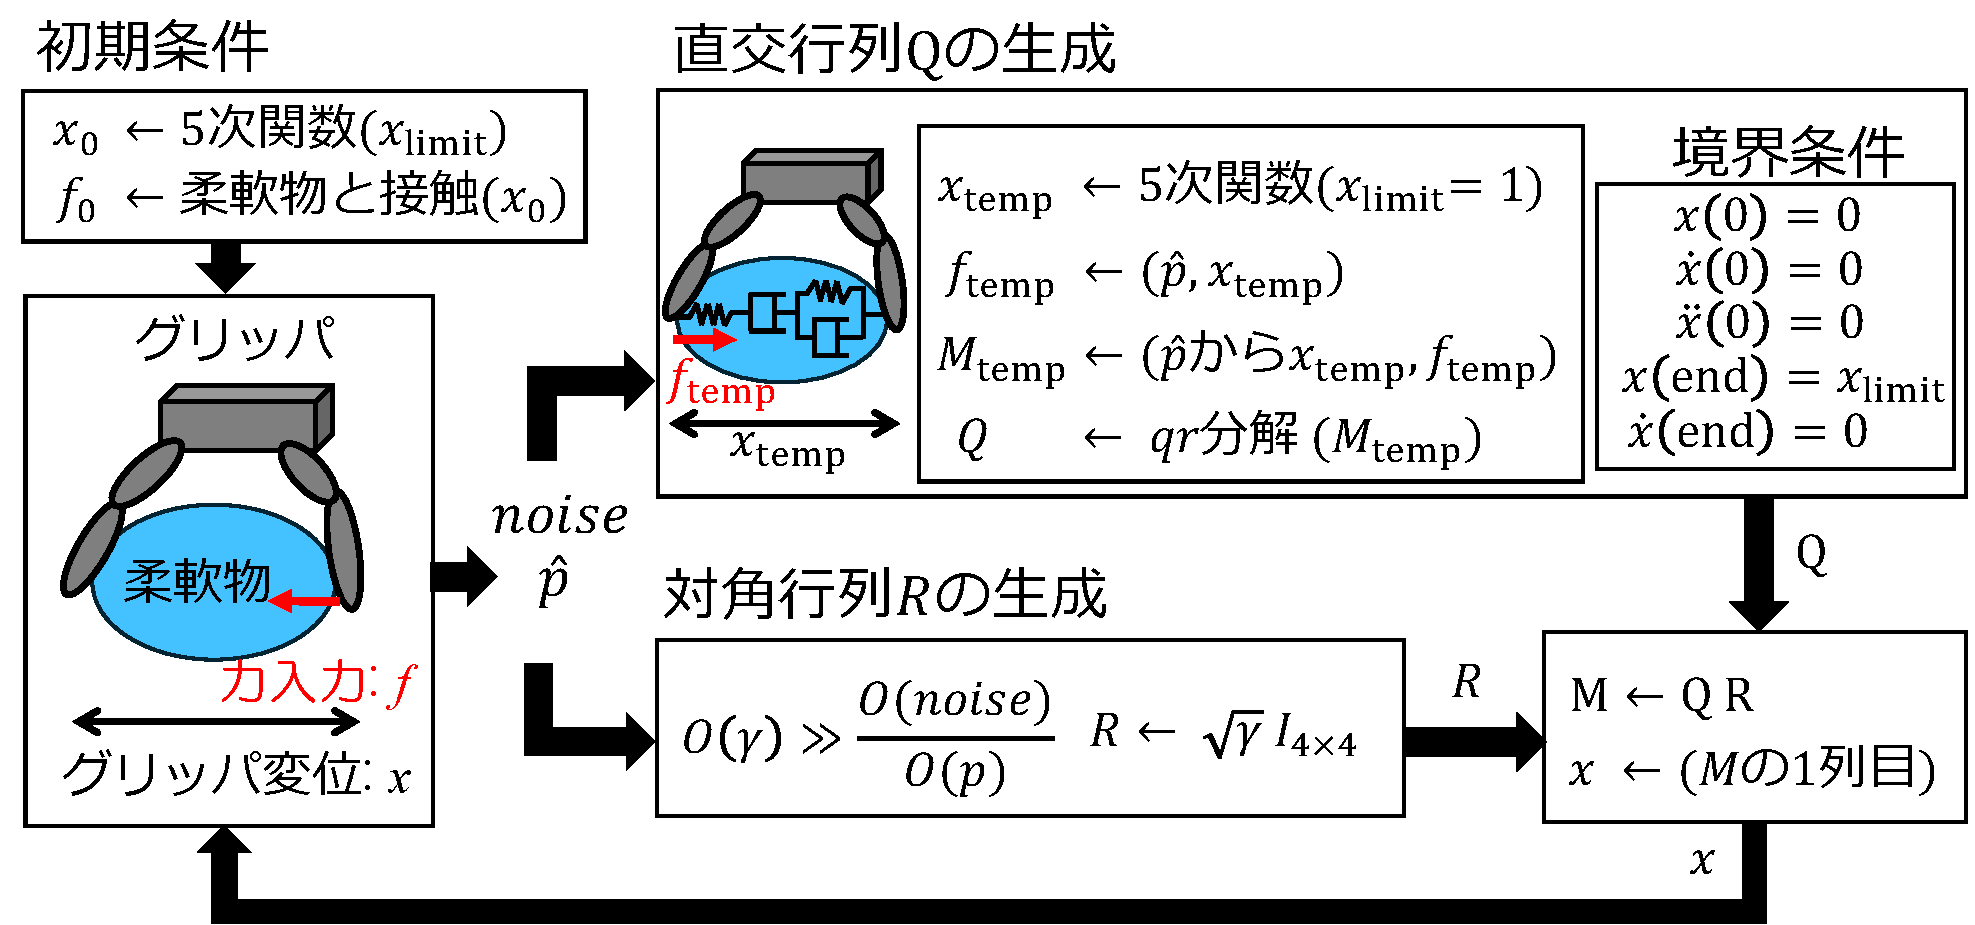
\includegraphics[width=0.48\textwidth]{QR_traj.pdf}
    \captionsetup{width=0.9\linewidth} % キャプションの幅をページ幅の90%に設定
    \caption{Generation of the gripper trajectory using QR decomposition.}
    \label{fig:QR_traj}
\end{figure}
直交行列$\mathbf{Q}$は,図~\ref{fig:QR_traj}の上側ルートで生成する.
$\mathbf{Q}$は$\mathbf{M}_{\mathrm{v}}$とは別の一時的な行列$\mathbf{M}_{\mathrm{temp}}$をQR分解することで得る.
$\mathbf{M}_{\mathrm{temp}}$は,1サイクル前に同定したパラメータ$\mathbf{p}$を柔軟物モデルに適応し,仮想的な5次関数形状の変形量$\boldsymbol{x}_{\mathrm{temp}}$を与えることで得られる.
% 1サイクル前に同定したパラメータ$\mathbf{p}$を柔軟物モデルに適応し,仮想的な5次関数形状の変形量$\boldsymbol{x}_{\mathrm{temp}}$を与えることで一時的な行列$\mathbf{M}_{\mathrm{temp}}$を得る.
% さらに,$\mathbf{M}_{\mathrm{temp}}$をQR分解することで$\mathbf{Q}$を得る.
対角行列$\mathbf{R}$は,図~\ref{fig:QR_traj}の下側ルートで生成し,
$\gamma$を対角成分とした$4\times4$行列とする.
最終的に,独立して得られた$\mathbf{Q}$と$\mathbf{R}$を掛け合わせることで,行列$\mathbf{M_{\mathrm{v}}}$を生成し,その1列目をグリッパの軌道$\boldsymbol{x}$とする.

最後に,このグリッパの軌道生成に適したパラメータ$\mathbf{p}$の計算方法について述べる.
粘弾性モデルの変形と反力の関係式~(\ref{eq:BSmodel})を行列式~(\ref{eq:Mp_q})(\ref{eq:BSmodel_matrix})に変形する際,
$\mathbf{q}$には$\boldsymbol{f}, \int{\boldsymbol{f}} , \iint{\boldsymbol{f}}, \boldsymbol{x} , \int{\boldsymbol{x}}$の5通りの選び方がある.上記で述べたグリッパの軌道は,$\mathbf{q}$のノイズの影響を抑える軌道になっており,
$\mathbf{q}$にもっともノイズの大きい$\boldsymbol{f}$を用いることで
提案した軌道生成が有効に働く.

%%%%%%%%%%%%%%%%%%%%%%%%%%%%%%%%%%%%%%%%%%%%%%%%%%%%%%%%%%%%%%%%%%%%%%%%%%%%%%%%%%%%%%%%%%%%%%%%%%%%%%%%%%%%%%%%%%%%%%%%%%%%%%%%%%%%%%%%%%%%%%%%%%%%%%%%%%%%%%%
\subsection{粘弾性係数の逐次的な値の更新方法}\label{subsec:downsample}
 粘弾性係数と$\boldsymbol{x}$,$\boldsymbol{f}$の関係式~(\ref{eq:Mp_q})は不能であり,求める解$\mathbf{p}$が4要素であるのに対し,方程式の数が過剰であり矛盾する式が含まれる.一部の矛盾する式より粘弾性係数が負になり,物理的に妥当性を失う場合がある.
そこで,式~(\ref{eq:Mp_q})の擬似逆行列の算出方法を逐次的に行い,粘弾性係数が物理的に妥当でないデータは除外する.
まず擬似逆行列の逐次的な算出方法について述べ,次に除外するデータの決定方法について述べる.

タイムステップが$n-1$までの行列$\mathbf{M}$を$\mathbf{M}_{n-1}$とし,$n$番目のタイムステップのデータ$\mathbf{m}_n$として,タイムステップ$n$での行列$\mathbf{M}_n$を,
\begin{equation}
    \begin{aligned}
        \mathbf{M}_n &= \begin{bmatrix}
            \mathbf{M}_{n-1} ,\mathbf{m}_n
        \end{bmatrix}^{T},\\
        \mathbf{m_{n}}&=\begin{bmatrix}
            x_{n} & \int{x_{n}} & -\int{f_{n}}\ & -\iint{f_{n}}\\
        \end{bmatrix}
    \end{aligned}
\end{equation}
とする.このとき$(\mathbf{M_{n}}^{T}\mathbf{M_{n}})^{-1}$を$\mathbf{J}_{n}$とし,$\mathbf{J}_{n}$の更新式はWoodburyの公式を用いて,
\begin{equation}
    \begin{aligned}
    \mathbf{J}_n &= (\mathbf{M_{n}}^{T}\mathbf{M_{n}})^{-1}\\
                 &= (\mathbf{M_{n-1}}^{T}\mathbf{M_{n-1}} + \mathbf{m_{n}}^{T}\mathbf{m_{n}})^{-1}\\
                 &= \mathbf{J}_{n-1} - \frac{\mathbf{J}_{n-1}\mathbf{m_{n}}\mathbf{m_{n}}^{T}\mathbf{J}_{n-1}}{1+\mathbf{m_{n}}^{T}\mathbf{J}_{n-1}\mathbf{m_{n}}}
    \end{aligned}
    \label{eq:step_J}
\end{equation}
と表せる.$\mathbf{p}$の$n-1$番目と$n$番目の関係は,
\begin{equation}
    \begin{aligned}
    \mathbf{p}_n &= (\mathbf{M_{n}}^{T}\mathbf{M_{n}})^{-1}\mathbf{M_{n}}^{T}\mathbf{q_{n}}\\
                 &= \mathbf{J}_{n}\mathbf{M_{n}}^{T}\mathbf{q_{n}}\\
                 &= \mathbf{J}_{n}(\mathbf{p}_{n-1}+\mathbf{m_{n}}^{T}\mathbf{q_{n}})\\
    \end{aligned}
    \label{eq:step_p}
\end{equation}
となる.この更新式~(\ref{eq:step_J}),~(\ref{eq:step_p})とタイムステップ$n$で計測されるデータ$\mathbf{m_{n}}$と$\mathbf{q_{n}}$を用いて$\mathbf{p}_{n\_temp}$を算出し,$\mathbf{p}_{n}$の更新に利用するか,除外するか判断する.

次に,除外するデータの決定方法について,式~(\ref{eq:p2ck})を変形し$\mathbf{p}$から$k_1$,$k_2$,$c_1$,$c_2$は,
\begin{equation}
    \begin{aligned}
        k_1 &= p_1 ,\\
        k_2 &= \frac{p_2}{p_3 - \frac{p_4 p_1}{p_2} - \frac{p_2}{p_1}} ,\\
        c_1 &= \frac{p_2}{p_4},\\
        c_2 &= \frac{p_1}{p_3 - \frac{p_4 p_1}{p_2} - \frac{p_2}{p_1}} 
    \end{aligned}
\end{equation}
のように算出できる.さらに,ゼロ除算や値の発散をさけるため,更新に用いる$\mathbf{p}_{n\_temp}=[p'_1,p'_2,p'_3,p'_4]^{T}$の条件は,
\begin{equation}
    \begin{aligned}
        10^{-7} < {p}'_{i} < 10^{7} ,\\
        10^{-7} < \left( p'_3 - \frac{p'_4 p'_1}{p'_2} - \frac{p'_2}{p'_1} \right)
    \end{aligned}
\end{equation}
とした.
これにより安定して物理的に妥当な粘弾性係数を算出できる.
%%%%%%%%%%%%%%%%%%%%%%%%%%%%%%%%%%%%%%%%%%%%%%%%%%%%%%%%%%%%%%%%%%%%%%%%%%%%%%%%%%%%%%%%%%%%%%%%%%%%%%%%%%%%%%%%%%%%%%%%%%%%%%%%%%%%%%%%%%%%%%%%%%%%%%%%%%%%%%
\section{評価実験}
\subsection{実験システム}
 実験に用いたグリッパと実験対象の柔軟物を図~\ref{fig:exp_setup}に示す.駆動系にはシャフトモータ (日本パルスモータ社製;SL083)を用い,1 kHzで制御した.
% ,ドライバ(Panasonic製,MADHT1107L01)を用いた.本システムは1 kHzの制御周期で動作した.
\begin{figure}[tb]
    \centering
    \includegraphics[width=0.45\textwidth]{exp_setup.pdf}
    \caption{Experimental setup and test object.}
    \label{fig:exp_setup}
\end{figure}
% windows PC上でグリッパの軌道を生成し,シリアル通信(RS422,ボートレート...)でdSPACE DS1104に送信し,dSPACEがシステム全体のリアルタイム制御を管理した.
反力の真値を確認するために,力センサ(レプトリノ社製;PFS030YA151G6)を用いた.
研修医の超音波ガイド下での処置の練習対象として,鶏むね肉や,豆腐,ゼラチンが用いられ,縫合の練習対象としてバナナ,豆腐,ゼラチンを用いる場合があることから\cite{exp_ref1}\cite{exp_ref2}\cite{exp_ref3},
実験対象として,鶏むね肉,豆腐,バナナを用いた.
%%%%%%%%%%%%%%%%%%%%%%%%%%%%%%%%%%%%%%%%%%%%%%%%%%%%%%%%%%%%%%%%%%%%%%%%%%%%%%%%%%%%%%%%%%%%%%%%%%%%%%%%%%%%%%%%%%%%%%%%%%%%%%%%%%%%%%%%%%%%%%%%%%%%%%%%%%%%%%%%.
\subsection{評価方法}
 1回の実験は15秒間で行い,はじめの6秒間を変形段階,次の9秒間を停止段階とした.
停止段階9秒ではグリッパに変形段階での最終値目標位置を与え続けた.
この変形段階6秒間で粘弾性係数($k_1, k_2, c_1, c_2$)を同定し,停止段階9秒間での反力を推定した.
推定反力は力センサの計測結果との平均絶対誤差(MAE: Mean Absolute Error)を算出し評価した.
実験では,2つのグリッパ軌道により反力推定精度を比較した.
1つ目は,提案手法による軌道であり,変形段階の6秒を2秒ごとの3サイクルに分割し生成した(Prop.;propused method).
もう1つは,提案手法と同じ最終値を持つ5次関数形状の軌道である(Quint.;quintic polynomial).
% 1つは,提案手法により生成したグリッパ軌道であり,もう1つは,それと同じ最終値を持つ5次関数形状の軌道である.
5次関数の境界条件は,図~{\ref{fig:QR_traj}}の直交行列の生成時に用いた境界条件と同じである.
%%%%%%%%%%%%%%%%%%%%%%%%%%%%%%%%%%%%%%%%%%%%%%%%%%%%%%%%%%%%%%%%%%%%%%%%%%%%%%%%%%%%%%%%%%%%%%%%%%%%%%%%%%%%%%%%%%%%%%%%%%%%%%%%%%%%%%%%%%%%%%%%%%%%%%%%%%%
\subsection{結果}
 図~\ref{fig:bar_result}に3つの対象物に対する推定反力のMAEを示す.すべての対象物において,提案手法により生成したグリッパ軌道の方が5次関数形状の軌道よりもMAEが小さく,反力推定精度が高いことがわかる.
図~\ref{fig:prop_quint}に鶏むね肉を対象とし,反力推定と力センサの計測結果を示す.提案手法は5次関数形状と比較して,反力の最大値と反力の減少傾向が力センサの計測結果と類似していることがわかる.
バナナと豆腐も同様な類似であった.
\begin{figure}[tb]
    \centering
    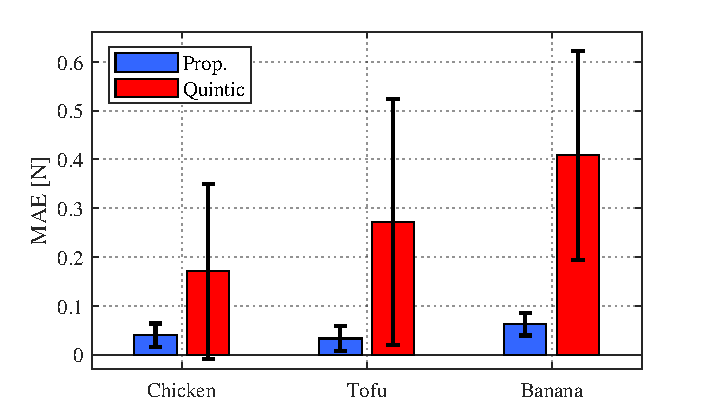
\includegraphics[width=0.5\textwidth]{bar_result.pdf}
    \caption{Bar result of MAE.}  
    \label{fig:bar_result}
\end{figure}
\begin{figure}[tb]
    \centering
    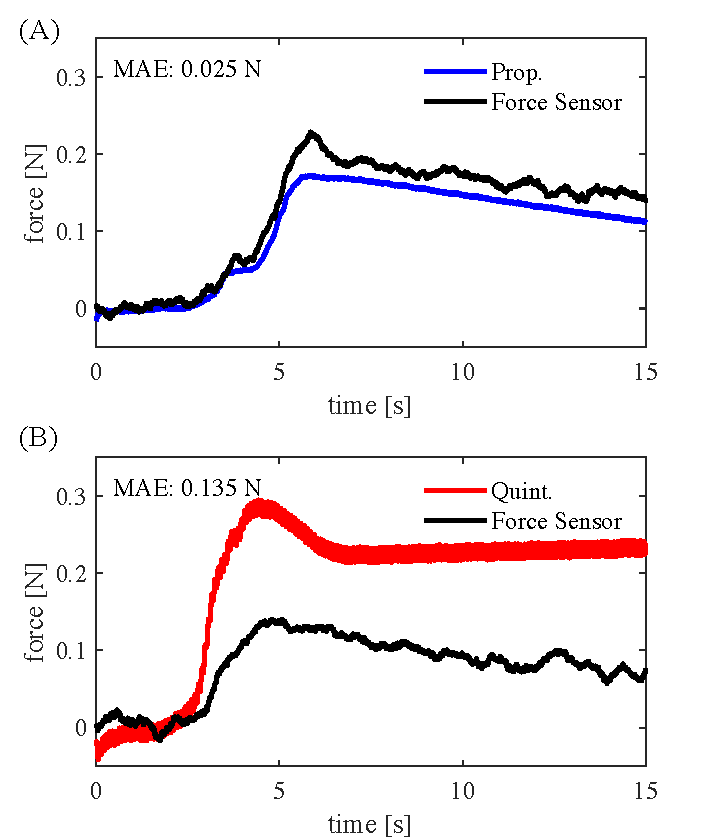
\includegraphics[width=0.5\textwidth]{prop_quint.pdf}
    \captionsetup{width=0.9\linewidth} % キャプションの幅をページ幅の90%に設定
    \caption{Compare prediction force with force sensor; (A) proposed method, (B) quintic polynomial.}
    \label{fig:prop_quint}
\end{figure}
%%%%%%%%%%%%%%%%%%%%%%%%%%%%%%%%%%%%%%%%%%%%%%%%%%%%%%%%%%%%%%%%%%%%%%%%%%%%%%%%%%%%%%%%%%%%%%%%%%%%%%%%%%%%%%%%%%%%%%%%%%%%%%%%%%%%%%%%%%%%%
\section{考察}
 提案手法の軌道生成は,1サイクルを2秒とし3サイクルで実験を行った.前サイクルで計測されたノイズと推定した粘弾性係数をもとに,次サイクルのグリッパ軌道を生成するため,
サイクルを重ねるごとに反力の推定精度が向上することが期待される.
図~\ref{fig:compare_cycle_MAE}に,対象物を豆腐とし,軌道生成のサイクルごとのMAEを示す.提案手法では,3サイクル目で推定反力のMAEが減少することがわかる.
一方で,5次関数形状の軌道では,変形過程の6秒間で推定反力のMAEの減少が見られない.
5次関数形状の軌道でMAEが減少しない原因は,\ref{subsec:downsample}節のデータの抽出により,変形過程の6秒間の大半のデータが粘弾性係数が物理的に妥当でないとして,除外されるためである.
2つの軌道のサイクルごとでのMAEの傾向は,残りの2つの対象物(鶏肉,バナナ)でも同様であった.
特異値に注目しサイクルごとに軌道を生成することは,単純な5次関数形状の軌道よりも,反力推定精度を向上させることができる.
\begin{figure}[t]
    \centering
    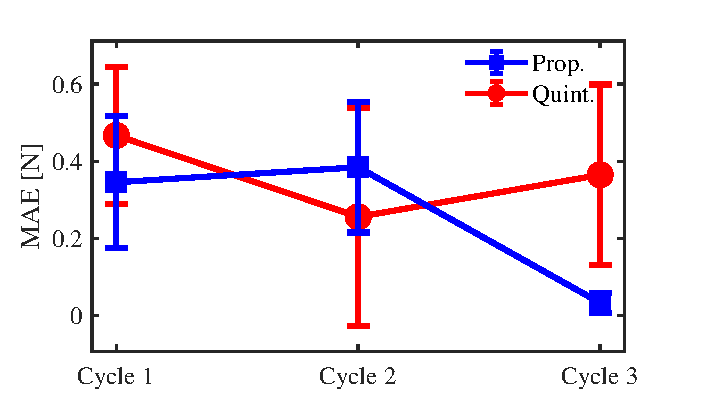
\includegraphics[width=0.5\textwidth]{compare_cycle_MAE.pdf}
    \caption{compare MAE among cycles (tofu)}
    \label{fig:compare_cycle_MAE}
\end{figure}

次に,\ref{subsec:QR_traj_and_calculation}節で述べた軌道に適した同定計算の有効性について考察する.
提案手法による軌道生成では,式~(\ref{eq:BSmodel_matrix})の$\mathbf{q}$に重畳したノイズの影響を抑えることを目的としており,
軌道に適した同定計算として,$\mathbf{q}$に最もノイズの大きい$\boldsymbol{f}$を用いることを提案した.
図~\ref{fig:compare_select5mode}に,対象物をバナナとし$\mathbf{q}$の選び方を変えた場合のMAEを示す.
$\mathbf{q}$に$\boldsymbol{f}$を用いた場合のMAEが最も小さく,$\boldsymbol{{f}}$に関しては,積分を重ねるごとにMAEが増加することがわかる.
よって,提案した同定計算は,グリッパの軌道に適しており,反力推定精度を向上させていることがわかる.
\begin{figure}[t]
    \centering
    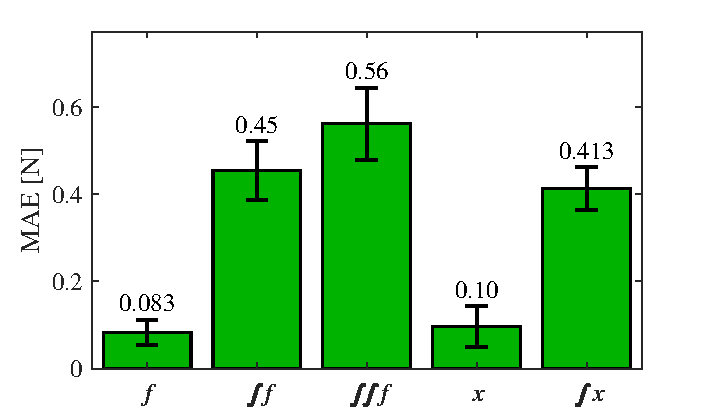
\includegraphics[width=0.5\textwidth]{select_differet_q_banana.pdf}
    \captionsetup{width=0.9\linewidth} % キャプションの幅をページ幅の90%に設定
    \caption{Compare 5 moethod of identification calculation (banana).}
    \label{fig:compare_select5mode}
\end{figure}
%%%%%%%%%%%%%%%%%%%%%%%%%%%%%%%%%%%%%%%%%%%%%%%%%%%%%%%%%%%%%%%%%%%%%%%%%%%%%%%%%%%%%%%%%%%%%%%%%%%%%%%%%%%%%%%%%%%%%%%%%
\section{結言}
%〇〇するために,XXを提案した.実験をもとに,CCを確認した.今後の展望として,
 本研究では,力センサを用いずに反力を推定する手法を提案した.
柔軟物の粘弾性係数をノイズにロバストに算出する課題を設定し,
グリッパの軌道生成と軌道に適した同定計算,粘弾性係数の更新方法を提案した.
実験により,提案手法により生成したグリッパの軌道を用いることで,5次関数形状の軌道よりも反力推定精度が向上することを確認した.
今後の展望として,柔軟物把持,柔軟物から異物を引き剥がす等の具体的なタスクをセンサレスで実現する\cite{future_work1}.
% \FloatBarrier
\begin{thebibliography}{9}
    %%勝手に設定
    \setlength{\itemsep}{0pt} % 各項目間の間隔を狭くする
    % \setlength{\parsep}{-2pt}  % 段落間の間隔を狭くする
    \renewcommand{\baselinestretch}{0.8}\selectfont % 行間を狭くする
    \setlength{\parskip}{0pt} % 段落の余白を狭くする
    %%勝手に設定ここまで
    % \bibitem{ref1}
    % 計測 太郎:センシングフォーラム予稿の書き方,第39回センシングフォーラム論文集,pp. 1-5, 2022.

    %%%%%%%MIS
    \bibitem{MIS_ref1}
    W. Wang, J. Wang, Y. Luo, X. Wang, H. Song:
    A Survey on Force Sensing Techniques in Robot-Assisted Minimally Invasive Surgery,
    IEEE Transactions on Haptics,pp.702–718, 2023.
    \bibitem{MIS_ref2}
    Zarrin PS, Escoto A, Xu R, Patel RV, Naish MD, Trejos AL: 
    Development of a 2-DOF sensorized surgical grasper for grasping and axial force measurements,
    IEEE Sensors Journal,pp.2816–2826, 2018.
    \bibitem{MIS_ref3}
    Okamura AM:
    Haptic feedback in robot-assisted minimally invasive surgery,Curr Opin Urol,pp.102–107, 2009.
    \bibitem{MIS_ref4}
    Lee C, Park YH, Yoon C, Noh S, Lee C, Kim Y, Kim HC, Kim HH, Kim S:
    A grip force model for the da Vinci end-effector to predict a compensation force,Med Biol Eng Comput,pp.253–261, 2015.

    \bibitem{MIS_ref5}
    Schostek S, Schurr MO, Buess GF:
    Review on aspects of artificial tactile feedback in laparoscopic surgery,Med Eng Phys,pp.887–898, 2009.

    
    %スペース的制約
    %{MIS_ref1}
    \bibitem{MIS_ref6}%生体適合性
    Trejos AL, Escoto A, Hughes D, Naish MD, Patel RV:
    A sterilizable force-sensing instrument for laparoscopic surgery,pp.157–162,2014.

    \bibitem{MIS_learning_time}%外科医の習得時間
    Shahzada KS, Yurkewich A, Xu R, Patel RV:
    Sensorization of a surgical robotic instrument for force sensing,pp.153–162,2016.
    
    \bibitem{MIS_ref7}%殺菌
    Trejos AL, Escoto A, Naish MD, Patel RV:
    Design and evaluation of a sterilizable force sensing instrument for minimally invasive surgery,IEEE Sensors Journal,pp.3983–3993, 2017.

    \bibitem{RMIS}%ロボット支援手術での力センサの必要性
    Amirabdollahian F, Livatino S, Vahedi B, Gudipati R, Sheen P, Gawrie-Mohan S, Vasdev N:
    Prevalence of haptic feedback in robot-mediated surgery: a systematic review of literature,Journal of robotic surgery,pp.11–25, 2018.





    %%%fps
    \bibitem{fps_ref1}%500 Hz
    Jones D, Wang H, Alazmani A, Culmer PR:
    A soft multi-axial force sensor to assess tissue properties in realtime,pp.5738–5743,2017.
    \bibitem{fps_ref2}%1 kHz
    Choi S, Tan HZ:
    Effect of update rate on perceived instability of virtual haptic texture,pp.3577–3582,2004.

    %%%related work
    \bibitem{ref_Chua}
    Chua Z, Jarc AM, Okamura AM:
    Toward force estimation in robot-assisted surgery using deep learning with vision and robot state,pp.12335–12341,2021.
    \bibitem{ref_Wang}
    Wang X, Ananthasuresh GK, Ostrowski JP:
    Vision-based sensing of forces in elastic objects,Sensors and Actuators A: Physical,pp.142–156, 2001.
    \bibitem{ref_Xue}
    Xue R, Du Z, Yan Z, Ren B:
    An estimation method of grasping force for laparoscope surgical robot based on the model of a cable-pulley system,
    Mechanism and Machine Theory,pp.440–454, 2019.


    \bibitem{ref_review_modeling}
    Yin H, Varava A, Kragic D:
    Modeling, learning, perception, and control methods for deformable object manipulation,Science Robotics,pp.eabd8803, 2021.
    \bibitem{ref_MSD}
    Ji W, Tang C, Xu B, He G:
    Contact force modeling and variable damping impedance control of apple harvesting robot,Comput Electron Agric,pp.107026, 2022.
    \bibitem{ref_PBD}
    Boonvisut P, Çavuşoğlu MC:
    Estimation of soft tissue mechanical parameters from robotic manipulation data,IEEE/ASME Transactions on Mechatronics,pp.1602–1611, 2012.
    \bibitem{ref_FEM}
    Lin H, Guo F, Wang F, Jia Y:
    Picking up a soft 3D object by “feeling” the grip,The International Journal of Robotics Research,pp.1361–1384, 2015.

    %%%%experimental onject
    \bibitem{exp_ref1}
    Kim YH:Ultrasound phantoms to protect patients from novices,The Korean journal of pain,pp. 73–77, 2016.
    \bibitem{exp_ref2}
    Wong K, Bhama PK, Mazimpaka Jd, Dusabimana R, Lee LN, Shaye DA:
    Banana fruit: an “appealing” alternative for practicing suture techniques in resource-limited settings, 
    Am J Otolaryngol,pp. 582–584, 2018.
    \bibitem{exp_ref3}
    Giannotti E, Jethwa K, Closs S, Sun R, Bhatti H, James J, Clarke C:
    Promoting simulation-based training in radiology: a homemade phantom for the practice of ultrasound-guided procedures,
    Br J Radiol,pp. 20220354, 2022.

    %%%%future work
    \bibitem{future_work1}
    川嶋健嗣: 
    低侵襲な外科手術を支援するロボットにおける力触覚センシング,日本ロボット学会誌,pp.405–408, 2019.




    

\end{thebibliography}

\end{document}

% end of sftemplate.tex